%----------------------------------------------------------------
\subsection{Hardware}
This section briefly describes the architecture of communication. In order to be versatile and flexible, the experiments will use one router and one WiFi adapter per quadrotor. The flexibility became because with those devices is don't restrict the software, i. e., the whole system can be uses with GSM modules and cloud computation or inside a computer with simulated targets and persecutors (Quadrotors).


%% 666 TODO: cambiar imagen a la que debe ser!!!
\begin{figure}[h]
	\begin{center}
		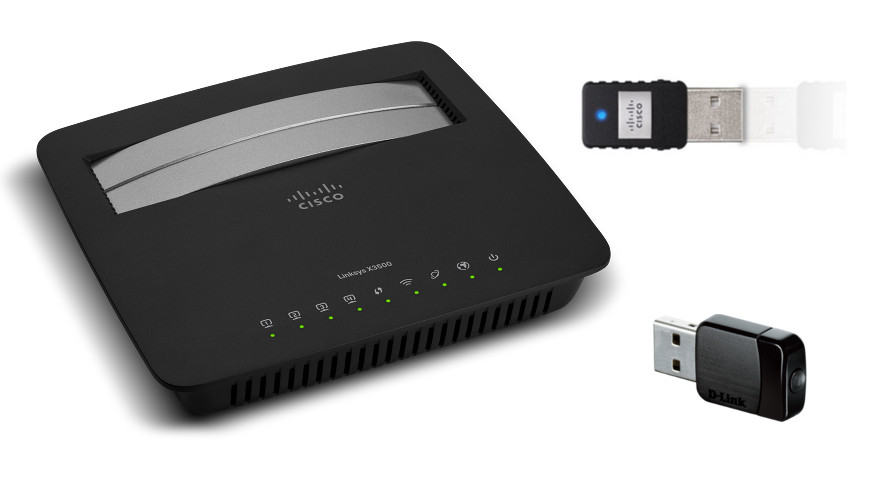
\includegraphics[width=0.5\textwidth]{../Images/c2/hardware_comm.jpg}
	\end{center}
	\caption{Hardware devices}
	\label{fig:hardware_comm}
\end{figure}

%----------------------------------------------------------------
\subsection{Software, protocol and messages}

To communicate between devices every application (or program) use a sockets \cite{SocketWiki}. Particularly, an implementation developed initially for this project that can be found in BOViL \cite{BOViL}. Sockets are configured with the TCP/IP protocol \cite{TCPIP}.

\begin{warpfigure}{r}{0.5\textwidth}
	\begin{center}
		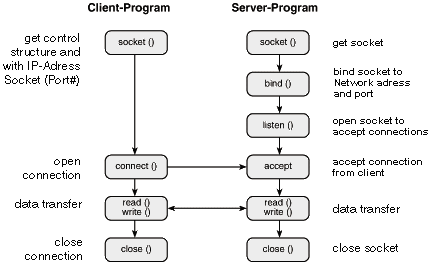
\includegraphics[width=0.5\textwidth]{../Images/c2/socketstcpip.jpg}
	\caption{Sockets and TCP-IP}
	\label{fig:socketstcpip}
\end{warpfigure}

